\section{What changes during a partial rollout?}\label{sec:rollout}
A service might try the new rule on a fraction of applicants and use the result to judge a full switch. We simulated that decision on the original 480 rental markets and two school cohorts. Independently for each applicant, we use policy $B$'s full menu with probability $p$ and otherwise keep $A$'s. We clear the entire market at each $p\in\{0,1/4,1/2,3/4,1\}$. We use 64 independent pairs of random assignments, with complementary uniforms within a pair and shared draws across uptake levels. This design gives a Monte Carlo standard error conditional on the fixed cohorts, preferences and candidate menus. For NYC we also resample whole simulation seed blocks. These experiments were specified after the original full-switch comparisons.

For any fixed reference offer, the expected number of people shown that offer is exactly the interpolation between the two endpoint counts: menu membership depends only on that person's switch. At half adoption the complementary assignments give that midpoint exactly in each pair. Placement need not follow the same line. For example, if two one-slot menus both show $x$ before the switch and both show $y$ afterward, either endpoint places one applicant. A mixed market with one applicant at each site places two. Reversing two initially distinct menus can bend the placement curve in the opposite direction.

\begin{figure}[ht]
\centering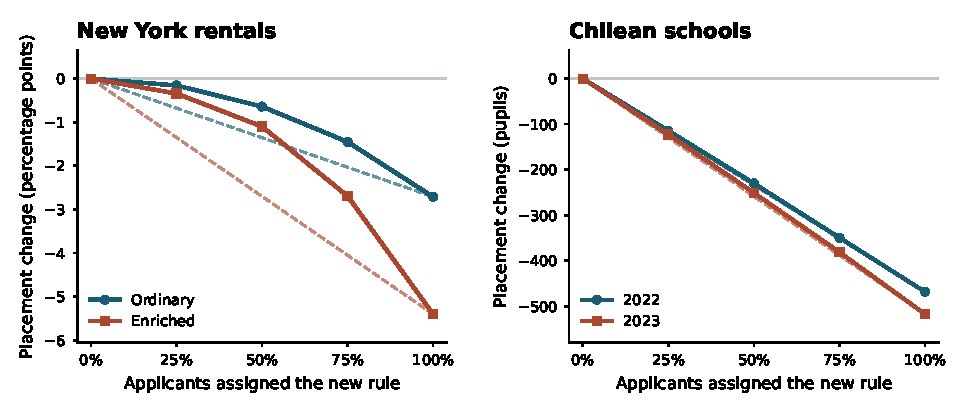
\includegraphics[width=.98\linewidth]{figures/adoption.pdf}
\caption{Placement change from the original policy when applicants independently switch to the proposed menu. Points give the simulated mean at each uptake. Dashed lines interpolate between full adoption and the original policy. The Chile panel reports pupils within each national cohort; the NYC panel uses geographically standardized percentage points.}
\Description{Placement declines in both markets. New York's mixed-policy outcomes sit above the straight-line interpolation by a larger proportion of the full-switch effect. The school curves lie close to their endpoint lines.}
\label{fig:uptake}\end{figure}

Placement at half adoption exceeded the interpolation by 0.71 and 1.60 percentage points in New York. The corresponding 95\% simulation-block intervals were $[0.59,0.84]$ and $[1.40,1.82]$, with Monte Carlo standard errors of 0.009 and 0.010 points. In Chile the midpoint deviation was about four pupils in 2022 and eight in 2023 (Monte Carlo standard errors 0.45 and 0.44 pupils, respectively). The school curves are close to linear in aggregate, yet applicants still change places. At half adoption an average of 272 pupils in 2022 and 271 in 2023 lost a place on a menu identical under both policies. The corresponding gains were 145 and 107. A nearly linear aggregate curve offers little protection to an individual family.

\section{Changing lists while protecting tentative offers}\label{sec:row-screen}

Suppose the platform observes an allocation $M_A$ stable on the old lists before deciding who receives new lists. Both menus retain the same underlying ranking over programs. Each person can receive either their entire old row $A_i$ or their entire proposed row $B_i$. Flag row $i$ if either (i) $M_A(i)$ is a real program missing from $B_i$, or (ii) $B_i$ contains a pair $(i,j)$ that would block $M_A$. For the second test, $i$ must prefer $j$ to $M_A(i)$, and $j$ must have a vacancy or prefer $i$ to one of its holders. Since $M_A$ is stable on $A$, only newly added options need this test. Let $F$ be the flagged applicants. With indexed rankings, check feasibility of each old contract and compute each program's occupancy and worst incumbent priority once. A scan of the proposed edges then constructs $F$ in linear time in the explicit menu and capacity input size. This rule uses baseline assignments and the rankings relevant to these pairs. In a simulation it can use the modeled rankings; a service with incomplete information would need to elicit these comparisons.

\begin{theorem}\label{thm:two-policy-screen}
If $S$ receives its proposed rows, $M_A$ remains stable exactly when $S\cap F=\varnothing$. On any such display every stable outcome has the original recipients, and applicant-proposing DA weakly improves every applicant's assignment relative to $M_A$. For an additive row objective with gain $g_i$ from switching row $i$, the largest net gain that keeps $M_A$ stable is $\sum_{i\notin F}(g_i)_+$.

More generally, put $R=S\cap F$ and let $N$ be any stable outcome on the mixed display. Let $K_j$ and $T_j$ count people in $R$ assigned to program $j$ under $M_A$ and $N$, respectively. The gross numbers of placement losses and gains are each at most
\[
 \bigl|\{i\in R: M_A(i)\ne\bot\text{ or }N(i)\ne\bot\}\bigr|-\sum_j\min(K_j,T_j)\ \leq\ |R|.
\]
\end{theorem}
\begin{proof}
A removed baseline partner makes $M_A$ infeasible. A newly displayed blocker prevents its stability. Both defects depend only on the applicant's row when the allocation being tested is fixed. In their absence every old contract survives and every displayed pair passes the blocking test. Matched-set invariance and applicant optimality give the first guarantees. The objective is therefore maximized by switching precisely the unflagged rows with positive gain, with free choice on zero gains.

For the bound, remove $R$ and its occupied seats from both allocations. In $M_A$ all remaining assignments survive on the mixed display and no remaining pair blocks. In $N$ stability also survives the restriction. Compare the resulting capacity vectors $c-K$ and $c-T$ using the one-seat argument of Theorem~\ref{thm:two-omission}. Outside $R$, losses are at most $\sum_j(T_j-K_j)_+$ and gains are at most $\sum_j(K_j-T_j)_+$. Within $R$, losses equal $\sum_j K_j-d$ and gains equal $\sum_j T_j-d$, where $d$ counts members matched under both allocations. Adding either margin yields the stated expression.
\end{proof}
The condition protects the old allocation as a stable witness. A flagged applicant can still switch without causing any placement loss. The distinction allows the rule to be checked before reallocation and limits the gains it can deliver. For independent switches with probabilities $p_i$, the probability that the old allocation remains stable is $\prod_{i\in F}(1-p_i)$, and expected gross losses or gains are at most $\sum_{i\in F}p_i$. The probability factorization is related to the one-sided uncertainty result of \citet{aziz_uncertain}. Here program priorities stay fixed and applicant menus change.

For a fixed reference partner, $g_i=C_i(B)-C_i(A)$. Maximizing this objective using the partner's identity gives a hindsight ceiling. In the 2022--23 school cohorts, 27,851 of 32,914 changed rows could switch together while supporting every old contract. Only 22 of the 3,750 newly shown full-list partners occurred on those rows. A platform could reasonably object: why choose between two complete lists when it can replace just one option? We address that objection next. Appendix~\ref{sec:rollout} separately studies random partial adoption without protection.

